\documentclass[UTF8,zihao=-4,a4paper]{ctexart}

\usepackage{geometry}
\usepackage{fontspec}
\usepackage{amsmath,amssymb}
\usepackage{booktabs}
\usepackage{tabularx}
\usepackage{longtable}
\usepackage{graphicx}
\usepackage{float}
\usepackage{caption}
\usepackage{subcaption}
\usepackage{enumitem}
\usepackage{xcolor}
\usepackage{hyperref}
\usepackage{url}
\usepackage{fancyhdr}
\usepackage{titlesec}

\geometry{left=2.5cm,right=2.5cm,top=2.6cm,bottom=2.6cm}
\IfFontExistsTF{Times New Roman}{\setmainfont{Times New Roman}}{\setmainfont{TeX Gyre Termes}}
\setlength{\parindent}{2em}
\setlength{\parskip}{0.2em}
\linespread{1.28}
\emergencystretch=2em
\graphicspath{{../}{./}}

\hypersetup{
  colorlinks=true,
  linkcolor=black,
  citecolor=black,
  urlcolor=blue,
  pdftitle={RetroAir：融合卫星 AOD 与气象数据的端到端历史 PM2.5 回顾性推断系统},
  pdfauthor={黄一和、夏浩博、黄迪、许君达}
}

\pagestyle{fancy}
\setlength{\headheight}{15pt}
\fancyhf{}
\fancyhead[C]{RetroAir 项目报告}
\fancyfoot[C]{\thepage}

\titleformat{\section}{\centering\heiti\zihao{3}}{\thesection}{0.8em}{}
\titleformat{\subsection}{\heiti\zihao{4}}{\thesubsection}{0.6em}{}
\titleformat{\subsubsection}{\heiti\normalsize}{\thesubsubsection}{0.5em}{}
\captionsetup{font=small,labelfont=bf}
\setlist{nosep,leftmargin=2em}

\newcommand{\pmfine}{PM$_{2.5}$}
\newcommand{\aod}{AOD}
\newcommand{\metric}[1]{\mathrm{#1}}

\begin{document}

\begin{titlepage}
  \centering
  \vspace*{2.6cm}
  {\zihao{1}\heiti RetroAir：融合卫星 AOD 与气象数据的端到端历史 PM2.5 回顾性推断系统\par}
  \vspace{1.2cm}
  {\zihao{3}\heiti 数据分析与数据挖掘期末项目报告\par}
  \vspace{2.2cm}
  {\zihao{4}选题类别：选项 C——端到端应用系统开发\par}
  \vspace{0.8cm}
  {\zihao{4}团队成员：黄一和、夏浩博、黄迪、许君达\par}
  \vfill
  {\zihao{4}2026 年 5 月\par}
\end{titlepage}

\begin{abstract}
地面空气质量监测站能够提供可靠的 \pmfine{} 浓度观测，但其空间覆盖受建设成本和维护条件限制，难以满足无站点地区历史暴露评估、环境健康研究和城市空气质量回顾分析的需求。针对这一问题，本文设计并实现了 RetroAir，一个融合卫星气溶胶光学厚度（Aerosol Optical Depth, \aod{}）与气象数据的端到端历史 \pmfine{} 回顾性推断系统。系统以 AKShare 真气网监测站数据作为监督标签，结合 CAMS EAC4 气溶胶再分析数据和 NASA POWER 日尺度气象数据，构建覆盖 2018--2025 年、中国 8 个城市、126 个监测站的多源融合数据集。方法上，系统形成了从数据获取、站点对齐、NetCDF 气溶胶特征提取、三源数据合并、特征标准化、模型训练、统一评估到 Web 推理应用的完整流水线。最终特征体系包含 9 个 \aod{} 特征、7 个气象特征和 1 个时间特征。

在模型层面，本文系统比较了 ResMLP、DCN-V2、CatBoost、LightGBM 和 XGBoost 等 5 类回归模型，并使用 10 个随机种子重复实验以降低单次随机切分带来的偶然性。实验结果表明，带 warmup 训练策略的残差多层感知机 ResMLP 在 8 城市 310,756 个样本上取得最优平均表现，测试集 $R^2$ 为 $0.8929\pm0.0031$，RMSE 为 $9.59\pm0.14\ \mu g/m^3$，MAE 为 $6.20\pm0.04\ \mu g/m^3$，Pearson 相关系数为 $0.945\pm0.002$。消融实验显示，气象+\aod{} 特征组合优于引入 OSM 空间特征或 MODIS RGB 反射率的扩展组合，说明本任务中动态气溶胶与气象变量已经提供了主要预测信息。系统最终通过 Streamlit 构建轻量级交互界面，支持地图选点、城市快捷选择、日期选择和一键 \pmfine{} 推理，完成了数据挖掘应用从数据到决策展示的闭环。

\noindent\textbf{关键词：} \pmfine{}；气溶胶光学厚度；多源数据融合；ResMLP；数据挖掘；端到端应用系统
\end{abstract}

\newpage
\tableofcontents
\newpage

\section{引言}

\pmfine{} 是空气污染暴露评估中最重要的颗粒物指标之一。世界卫生组织空气质量指南指出，细颗粒物长期暴露与呼吸系统、心血管系统等健康风险密切相关\cite{who2021}。在城市治理、公共卫生研究和环境流行病学中，连续、可靠且具有空间覆盖能力的 \pmfine{} 数据是分析污染暴露和制定政策的基础。然而，地面监测站虽然精度较高，却通常集中于人口密集和行政等级较高的城市区域。我国国控空气站点在“十三五”期间为 1,436 个，“十四五”期间优化为 1,734 个，仍难以覆盖广大农村、中小城市和城市边缘区\cite{mee2020}。因此，如何利用可公开获取的多源数据推断无监测站地区的历史 \pmfine{} 浓度，是一个具有现实意义的数据挖掘问题。

卫星遥感和大气再分析数据为该问题提供了新的数据基础。已有研究表明，卫星观测或再分析得到的 \aod{} 与地面 \pmfine{} 存在统计关联\cite{xin2016,zheng2017}，而温度、湿度、风速、气压、降水和云量等气象变量会影响颗粒物的扩散、吸湿增长与沉降过程。NASA 的空气质量与健康遥感综述也指出，卫星监测可作为地面站点的补充，用于改善空气质量空间覆盖\cite{holloway2023}。CAMS EAC4 再分析数据提供 2003 年至今的全球气溶胶产品\cite{cams}，NASA POWER 则提供面向能源和环境研究的全球日尺度气象数据接口\cite{nasa_power}，二者共同为历史 \pmfine{} 回顾性推断提供了可复现的数据来源。

本文项目 RetroAir 选择“端到端应用系统开发”方向，目标不是仅完成单个模型训练，而是构建一个完整的数据挖掘应用。系统从地面监测站标签出发，融合气象和 \aod{} 数据，训练回归模型并进行多算法对比，最后通过轻量级 Web 界面向用户提供任意经纬度与历史日期的 \pmfine{} 估计结果。本文贡献可概括为以下四点：

\begin{enumerate}
  \item 构建了覆盖数据获取、清洗、融合、特征生成、训练与推理的端到端流水线；
  \item 设计了由 9 个 \aod{} 特征、7 个气象特征和 1 个日期编码组成的 17 维特征体系；
  \item 对 ResMLP、DCN-V2、CatBoost、LightGBM 和 XGBoost 进行统一实验比较，并通过消融实验验证特征选择的合理性；
  \item 实现了基于 Streamlit 的交互式推理应用，将模型预测结果转化为可查看、可操作的空气质量信息。
\end{enumerate}

\section{相关工作与数据来源}

\subsection{相关研究}

利用遥感数据估计地面颗粒物浓度是环境数据挖掘和遥感反演中的典型问题。Xin 等\cite{xin2016}基于观测数据分析了中国区域 \pmfine{} 与 \aod{} 的关系，指出二者的关联受到相对湿度、边界层高度和气溶胶垂直分布等因素影响。Zheng 等\cite{zheng2017}进一步分析了北京地区 \pmfine{}--\aod{} 关系中的影响因素，表明气象条件在解释二者关系时不可忽略。Wei 等\cite{wei2019}使用时空随机森林估计中国 1 km 分辨率 \pmfine{} 浓度，说明机器学习模型能够有效融合遥感、气象和时空变量。Li 等\cite{li2017}则从城市公开数据挖掘角度研究细粒度 \pmfine{} 建模，体现了公共数据源在城市空气质量建模中的应用价值。

与上述研究相比，RetroAir 更强调课程项目要求中的工程闭环：在保证建模效果的同时，完整实现数据管道、模型训练、评估可视化和交互式推理界面。因此，本文既关注模型效果，也关注系统可复现性、模块划分和面向用户的部署形态。

\subsection{数据来源}

本项目使用三类核心数据源，见表\ref{tab:data_source}。其中，\pmfine{} 标签来自 AKShare 真气网监测站接口，包含 2018--2025 年中国 8 个城市、126 个站点的逐日空气质量记录；气象特征来自 NASA POWER API，提供 0.5° 日尺度气象变量；气溶胶特征来自 CAMS EAC4 再分析产品，空间分辨率为 0.75°，覆盖 2003 年至今。

\begin{table}[H]
  \centering
  \caption{RetroAir 使用的数据来源}
  \label{tab:data_source}
  \small
  \begin{tabularx}{\textwidth}{lllX}
    \toprule
    数据类型 & 来源 & 分辨率 & 覆盖范围 \\
    \midrule
    空气质量标签（\pmfine{}） & AKShare 真气网监测站 & 站点级 & 2018--2025，中国 8 城 126 站 \\
    气象数据 & NASA POWER API & 0.5° 日均 & 全球，实时 \\
    气溶胶 \aod{} & CAMS EAC4 再分析 & 0.75° 日均 & 全球，2003 年至今 \\
    \bottomrule
  \end{tabularx}
\end{table}

上述数据源具有明显互补性：地面站点提供可信监督标签，气象数据反映污染物扩散与沉降条件，\aod{} 数据则从大气气溶胶角度提供区域尺度的遥感代理变量。三者融合后，模型能够学习从“气象--气溶胶--地面颗粒物”到 \pmfine{} 浓度的统计映射。

\section{系统总体设计}

\subsection{端到端流程}

RetroAir 的总体架构如图\ref{fig:pipeline}所示。系统以站点、日期和经纬度为基本索引，将不同来源的数据对齐到日尺度样本。训练阶段先构建多源融合数据集，再进行特征标准化、随机切分、模型训练和评估；推理阶段由用户输入经纬度和日期，系统在线获取气象特征，从本地 CAMS NetCDF 文件提取 \aod{} 特征，加载训练好的 ResMLP 模型输出 \pmfine{} 预测值和空气质量等级。

\begin{figure}[H]
  \centering
  \fbox{
  \begin{minipage}{0.93\textwidth}
  \centering
  \vspace{0.5em}
  AKShare 监测站 \pmfine{} 标签
  \quad+\quad NASA POWER 气象数据
  \quad+\quad CAMS EAC4 \aod{} 数据

  \vspace{0.7em}
  $\Downarrow$

  \vspace{0.7em}
  站点坐标对齐 $\rightarrow$ 日尺度特征提取 $\rightarrow$ 三源 inner join $\rightarrow$ 17 维特征矩阵

  \vspace{0.7em}
  $\Downarrow$

  \vspace{0.7em}
  多模型训练与评估 $\rightarrow$ ResMLP 最优模型保存 $\rightarrow$ Streamlit 交互式推理应用
  \vspace{0.5em}
  \end{minipage}}
  \caption{RetroAir 端到端系统流程}
  \label{fig:pipeline}
\end{figure}

\subsection{代码模块与职责}

项目采用模块化脚本组织。数据构建入口为 \path{00_build_dataset.py}，其依次调度 AQI 获取、气象获取、\aod{} 提取和数据合并脚本；模型对比入口为 \path{06_compare_algorithms.py}；推理逻辑由 \path{inference.py} 封装，供命令行和 Web 应用复用。核心模块见表\ref{tab:modules}。

\begin{table}[H]
  \centering
  \caption{RetroAir 主要模块}
  \label{tab:modules}
  \begin{tabularx}{\textwidth}{lX}
    \toprule
    模块 & 功能 \\
    \midrule
    \texttt{01\_fetch\_aqi.py} & 获取真实监测站 \pmfine{} 标签，并关联公开站点坐标清单 \\
    \texttt{02\_fetch\_weather.py} & 按站点经纬度获取 NASA POWER 日尺度气象数据 \\
    \texttt{03\_fetch\_aod.py} & 从 CAMS EAC4 NetCDF 文件中按经纬度和日期提取 \aod{} 特征 \\
    \texttt{04\_merge\_data.py} & 以城市、站点、日期为键合并 AQI、气象与 \aod{} 三源数据 \\
    \texttt{06\_compare\_algorithms.py} & 统一训练并比较 ResMLP、DCN-V2、CatBoost、LightGBM 和 XGBoost \\
    \texttt{app.py} & 基于 Streamlit 和地图组件提供交互式 \pmfine{} 推理界面 \\
    \bottomrule
  \end{tabularx}
\end{table}

该结构将数据工程、模型训练、评估和应用展示解耦，满足端到端应用系统对“可运行完整代码、模块化、有评估和交互界面”的交付要求。

\subsection{系统运行与复现路径}

从端到端应用系统的角度，RetroAir 的复现路径分为数据构建、模型训练和应用运行三个层次。数据构建层面，本项目算法流程以单城市为基本构建单元：先通过 \path{00_build_dataset.py} 按年份和城市构建 AQI、气象与 \aod{} 三源数据，再通过 \path{05_merge_to_final.py} 合并多城市数据集。该过程对应数据挖掘项目中的数据获取、清洗、特征抽取和数据集成阶段。

模型训练层面，\path{06_compare_algorithms.py} 是统一的算法对比入口。该入口在同一数据集、同一特征集合和相同评估指标下比较多类模型，并输出模型权重、指标文件和对比图。这样的组织方式避免了不同模型在数据预处理、切分方式或指标定义上不一致，保证实验结果可横向比较。应用运行层面，用户可通过 \texttt{streamlit run app.py} 启动轻量级 Web 界面，完成地图选点、日期选择、特征获取、模型推理和结果展示。

上述复现路径体现了“从数据到决策”的完整链条：原始数据经过脚本化处理形成训练集，训练集经过统一实验框架产生可部署模型，部署模型再通过交互式界面转化为用户可理解的 \pmfine{} 浓度和空气质量等级。这也是本文区别于单纯算法实验报告的关键所在。

\section{数据处理与特征工程}

\subsection{数据融合过程}

数据融合以 $(city, station\_name, date)$ 为主键，核心步骤如下：

\begin{enumerate}
  \item \textbf{站点标签获取：}按城市和日期抓取监测站空气质量数据，将 \pmfine{} 作为监督学习标签，并保留 PM10、NO$_2$、O$_3$ 等辅助字段用于数据记录；
  \item \textbf{站点坐标对齐：}将监测站名称标准化，关联公开站点经纬度清单，得到可用于气象和 \aod{} 查询的空间坐标；
  \item \textbf{气象数据获取：}对每个站点调用 NASA POWER 日尺度接口，获取温度、湿度、风速、风向、气压、降水和云量；
  \item \textbf{\aod{} 特征提取：}加载 CAMS EAC4 NetCDF 文件，按日期选择日内多个时次并求均值，再按最近网格点提取站点位置的气溶胶变量；
  \item \textbf{三源合并与清洗：}对 AQI、气象和 \aod{} 数据执行 inner join，删除标签或核心特征缺失的样本，并添加年内日序号作为时间编码。
\end{enumerate}

这一处理流程使最终样本既包含地面真实标签，也包含能够推广到无站点位置的外部环境特征。由于系统目标是对任意经纬度进行历史 \pmfine{} 回顾推断，模型输入不能依赖仅在监测站可得的污染物观测变量，而应使用可由全球数据源获取的气象与 \aod{} 特征。

\subsection{数据质量控制}

多源数据融合的主要风险在于时间粒度、空间坐标和字段含义不一致。RetroAir 在数据处理阶段采用三类质量控制策略。第一，所有数据统一到日尺度，并以标准日期字符串作为合并键，避免同一站点不同数据源因时间格式差异而错配。第二，站点名称在匹配前进行规范化处理，并保留站点经纬度，使气象和 \aod{} 查询能够以同一空间位置为基础。第三，在最终合并阶段，对标签缺失以及核心气象、\aod{} 特征缺失的样本进行剔除，确保进入模型训练的数据具有完整的监督学习结构。

这种质量控制并不改变本实验的数据规模和结果口径，而是保证三源数据能够被解释为同一“站点--日期”观测样本。对于回顾性 \pmfine{} 推断任务而言，数据对齐质量直接影响模型学习到的关系是否真实。如果 \aod{} 网格、气象网格和地面站点在日期或位置上错配，模型可能会学习到虚假的统计相关性。因此，数据质量控制是整个系统中与算法同等重要的部分。

\subsection{特征体系}

最终模型采用 17 维特征，分为 \aod{}、气象和时间三组。特征列表见表\ref{tab:features}。

\begin{table}[H]
  \centering
  \caption{最终采用的 17 维特征体系}
  \label{tab:features}
  \small
  \begin{tabularx}{\textwidth}{lcX}
    \toprule
    特征组 & 数量 & 变量及含义 \\
    \midrule
    \aod{} & 9 &
    \begin{tabular}[t]{@{}l@{}}
      \texttt{aod\_550}, \texttt{aod\_469}, \texttt{aod\_865}, \texttt{ae\_469\_865} \\
      \texttt{dust\_aod}, \texttt{sulphate\_aod}, \texttt{bc\_aod}, \texttt{om\_aod}, \texttt{ss\_aod} \\
      总气溶胶光学厚度、波长指数及沙尘、硫酸盐、黑碳、有机物、海盐等组分
    \end{tabular} \\
    气象 & 7 &
    \begin{tabular}[t]{@{}l@{}}
      \texttt{temperature\_2m\_mean}, \texttt{relative\_humidity\_2m\_mean} \\
      \texttt{wind\_speed\_10m\_mean}, \texttt{wind\_direction\_10m\_dominant} \\
      \texttt{surface\_pressure\_mean}, \texttt{precipitation\_sum}, \texttt{cloud\_cover\_mean} \\
      影响颗粒物扩散、沉降和吸湿增长的日尺度气象条件
    \end{tabular} \\
    时间 & 1 & \texttt{day\_of\_year}：年内日序号，用于刻画季节性变化 \\
    \bottomrule
  \end{tabularx}
\end{table}

其中，\texttt{ae\_469\_865} 为 469 nm 与 865 nm 两个波段之间的 Angstrom 指数，用于描述气溶胶粒径相关信息，其计算形式为
\begin{equation}
  AE_{469,865} = -\frac{\ln(AOD_{469}/AOD_{865})}{\ln(469/865)}.
  \label{eq:angstrom}
\end{equation}
当两个波段 \aod{} 均为正值时，该指标能够补充总 \aod{} 难以表达的粒径差异信息。

\subsection{特征消融}

项目初期曾考虑引入 OSM 空间特征和 MODIS RGB 地表反射率特征。根据本项目消融实验，在北京数据集上进行按监测站划分的 5 折交叉验证后，气象+\aod{} 组合取得最佳结果，$R^2=0.9089$，RMSE 为 9.40；加入 OSM 后 $R^2$ 降至 0.8979，加入 RGB 后 $R^2$ 降至 0.8967，同时加入二者后进一步降至 0.8883。OSM 和 RGB 单独使用时 $R^2$ 分别仅为 0.1906 和 0.1498。主要结果见表\ref{tab:ablation}。

\begin{table}[H]
  \centering
  \caption{特征组合消融实验结果}
  \label{tab:ablation}
  \begin{tabular}{lccc}
    \toprule
    特征组合 & $R^2$ & RMSE & 特征数 \\
    \midrule
    气象+\aod{} & 0.9089 & 9.40 & 17 \\
    气象+\aod{}+OSM & 0.8979 & 9.98 & 28 \\
    气象+\aod{}+RGB & 0.8967 & 10.06 & 27 \\
    气象+\aod{}+OSM+RGB & 0.8883 & 10.50 & 38 \\
    OSM 单独 & 0.1906 & 28.93 & 12 \\
    RGB 单独 & 0.1498 & 29.63 & 11 \\
    \bottomrule
  \end{tabular}
\end{table}

这一结果说明，静态土地利用代理和地表反射率变量并未提升本任务中的 \pmfine{} 回顾推断能力。可能原因在于，\pmfine{} 日尺度变化主要由气溶胶状态和气象过程驱动，而 OSM 特征缺少时间变化，MODIS RGB 更直接反映地表而非大气颗粒物。因此，最终系统保留“气象+\aod{}+时间”的紧凑特征组合。

\section{模型方法}

\subsection{问题定义}

给定样本 $i$ 的特征向量 $\mathbf{x}_i \in \mathbb{R}^{17}$，其中包含 \aod{}、气象和时间变量，模型目标是学习一个回归函数 $f_{\theta}$，使预测值 $\hat{y}_i=f_{\theta}(\mathbf{x}_i)$ 尽可能接近地面站点观测的 \pmfine{} 浓度 $y_i$：
\begin{equation}
  \hat{y}_i = f_{\theta}(\mathbf{x}_i), \quad
  y_i \in \mathbb{R}_{\geq 0}.
  \label{eq:regression}
\end{equation}

训练前，对输入特征进行标准化处理：
\begin{equation}
  x'_{ij} = \frac{x_{ij}-\mu_j}{\sigma_j},
  \label{eq:standardize}
\end{equation}
其中 $\mu_j$ 和 $\sigma_j$ 分别为训练集中第 $j$ 个特征的均值和标准差。对于深度模型，标签同样进行 z-score 标准化，推理后再映射回原始 \pmfine{} 尺度。

\subsection{ResMLP 模型}

最终部署模型为 ResMLP，即带残差结构的多层感知机。其结构包括输入投影层、多个残差块和回归头。输入投影层将 17 维特征映射到 128 维隐藏空间；每个残差块由线性层、ReLU、Dropout 和线性层组成，并通过 LayerNorm 稳定训练：
\begin{equation}
  \mathbf{h}_{l+1} = \mathrm{LayerNorm}\left(\mathbf{h}_{l} + g_l(\mathbf{h}_{l})\right).
  \label{eq:resblock}
\end{equation}
残差连接缓解了深层 MLP 在表格数据上的优化困难，使模型能够学习非线性特征交互，同时保持参数量较低。本项目最终 ResMLP 模型参数量约为 144K。

训练时采用 AdamW 优化器、SmoothL1Loss 损失函数、warmup 与余弦衰减学习率调度，并基于验证集早停。SmoothL1Loss 相比均方误差对异常值更稳健，适合 \pmfine{} 分布中可能存在的极端污染样本。

\subsection{对比模型}

为了系统评估模型选择，项目同时实现了树模型和深度学习模型：
\begin{itemize}
  \item \textbf{CatBoost：}基于梯度提升决策树，对非线性关系和特征交互具有较强建模能力；
  \item \textbf{LightGBM：}高效的梯度提升树模型，适合结构化表格数据；
  \item \textbf{XGBoost：}经典梯度提升框架，作为强基线模型；
  \item \textbf{DCN-V2：}通过显式 Cross Network 和深层网络并行建模特征交叉；
  \item \textbf{ResMLP：}通过残差 MLP 学习标准化后的连续变量非线性关系。
\end{itemize}

项目中还实现了 FT-Transformer 训练入口，但本次统一对比实验主要报告上述 5 个模型。后续实验结果均基于该模型对比口径展开。

\section{实验设置}

\subsection{数据集与切分}

根据本实验数据，模型对比实验使用 8 城市 310,756 个样本，采用随机切分方式进行训练与测试评估。选择随机切分而非时间切分，是因为本项目核心任务是历史 \pmfine{} 回顾性推断和空间补全，而不是未来时间序列预测。换言之，系统希望在已有历史气象与 \aod{} 条件下估计某位置的历史 \pmfine{} 浓度，因此随机切分能够评估模型在整体历史分布上的拟合和泛化能力。

同时，特征消融实验在北京数据集上采用站点切分的 5 折交叉验证，用于检验不同特征组在空间外推场景中的贡献。该设计能够减少同一站点时间序列泄漏对特征选择结论的影响。

\subsection{评估指标}

项目采用多指标评估回归模型，覆盖拟合优度、绝对误差、相对误差和相关性。主要指标定义如下。

决定系数：
\begin{equation}
  R^2 = 1 - \frac{\sum_i (y_i-\hat{y}_i)^2}{\sum_i (y_i-\bar{y})^2}.
  \label{eq:r2}
\end{equation}

均方根误差：
\begin{equation}
  RMSE = \sqrt{\frac{1}{n}\sum_i (y_i-\hat{y}_i)^2}.
  \label{eq:rmse}
\end{equation}

平均绝对误差：
\begin{equation}
  MAE = \frac{1}{n}\sum_i |y_i-\hat{y}_i|.
  \label{eq:mae}
\end{equation}

对称平均绝对百分比误差：
\begin{equation}
  SMAPE = \frac{100\%}{n}\sum_i \frac{2|y_i-\hat{y}_i|}{|y_i|+|\hat{y}_i|+\epsilon}.
  \label{eq:smape}
\end{equation}

其中，SMAPE 相比普通 MAPE 对接近零的 \pmfine{} 样本更稳健。项目还计算 Pearson 相关系数和 Explained Variance，用于衡量预测值与真实值的线性一致性和方差解释能力。

\subsection{实验可比性控制}

为了使模型对比具有学术意义，实验设计需要控制除模型结构以外的主要变量。根据本项目实验设计，统一对比实验使用相同的 17 维输入特征、相同的 8 城市样本集合、相同的随机切分策略和相同的回归指标体系。为降低单次随机切分和模型初始化带来的偶然性，本文使用 10 个随机种子（42--51）重复实验，并报告各指标的均值和标准差。树模型和神经网络模型虽然训练机制不同，但最终均在测试集原始 \pmfine{} 尺度上报告 $R^2$、RMSE、MAE 和 SMAPE，因此表\ref{tab:model_compare}中的数值具有可比性。

此外，消融实验与模型对比实验承担不同角色。模型对比实验回答“在最终特征体系下哪类算法表现最好”；消融实验回答“为何最终特征体系不引入 OSM 和 MODIS RGB”。前者使用 8 城市 310,756 样本随机切分结果，后者使用北京数据集上的站点切分 5 折交叉验证。两者评价目标不同，但共同支撑最终系统选择：输入采用气象+\aod{}+时间，部署模型采用 ResMLP。

\section{实验结果与分析}

\subsection{多算法对比}

表\ref{tab:model_compare}展示了 8 城市统一模型对比结果。ResMLP 在所有主要指标上表现最好，10 个随机种子的平均 $R^2$ 达到 0.8929，平均 RMSE 为 9.59 $\mu g/m^3$，平均 MAE 为 6.20 $\mu g/m^3$，平均 SMAPE 为 21.9\%。CatBoost、DCN-V2 和 LightGBM 的平均 $R^2$ 接近 0.81，XGBoost 相对较低。

\begin{table}[H]
  \centering
  \caption{8 城市 310,756 样本上的 10 随机种子模型对比结果}
  \label{tab:model_compare}
  \begin{tabular}{lccccc}
    \toprule
    模型 & $R^2$ & RMSE & MAE & SMAPE(\%) & 参数量 \\
    \midrule
    ResMLP (warmup) & \textbf{0.8929$\pm$0.0031} & \textbf{9.59$\pm$0.14} & \textbf{6.20$\pm$0.04} & \textbf{21.9$\pm$0.1} & 144K \\
    CatBoost & 0.8146$\pm$0.0034 & 12.61$\pm$0.12 & 8.40$\pm$0.02 & 27.3$\pm$0.1 & -- \\
    DCN-V2 & 0.8132$\pm$0.0042 & 12.66$\pm$0.12 & 8.22$\pm$0.03 & 27.0$\pm$0.1 & 48K \\
    LightGBM & 0.8119$\pm$0.0032 & 12.70$\pm$0.11 & 8.53$\pm$0.03 & 27.8$\pm$0.1 & -- \\
    XGBoost & 0.7727$\pm$0.0037 & 13.96$\pm$0.11 & 9.29$\pm$0.03 & 29.5$\pm$0.1 & -- \\
    \bottomrule
  \end{tabular}
\end{table}

\IfFileExists{../comparison_chart.png}{
\begin{figure}[H]
  \centering
  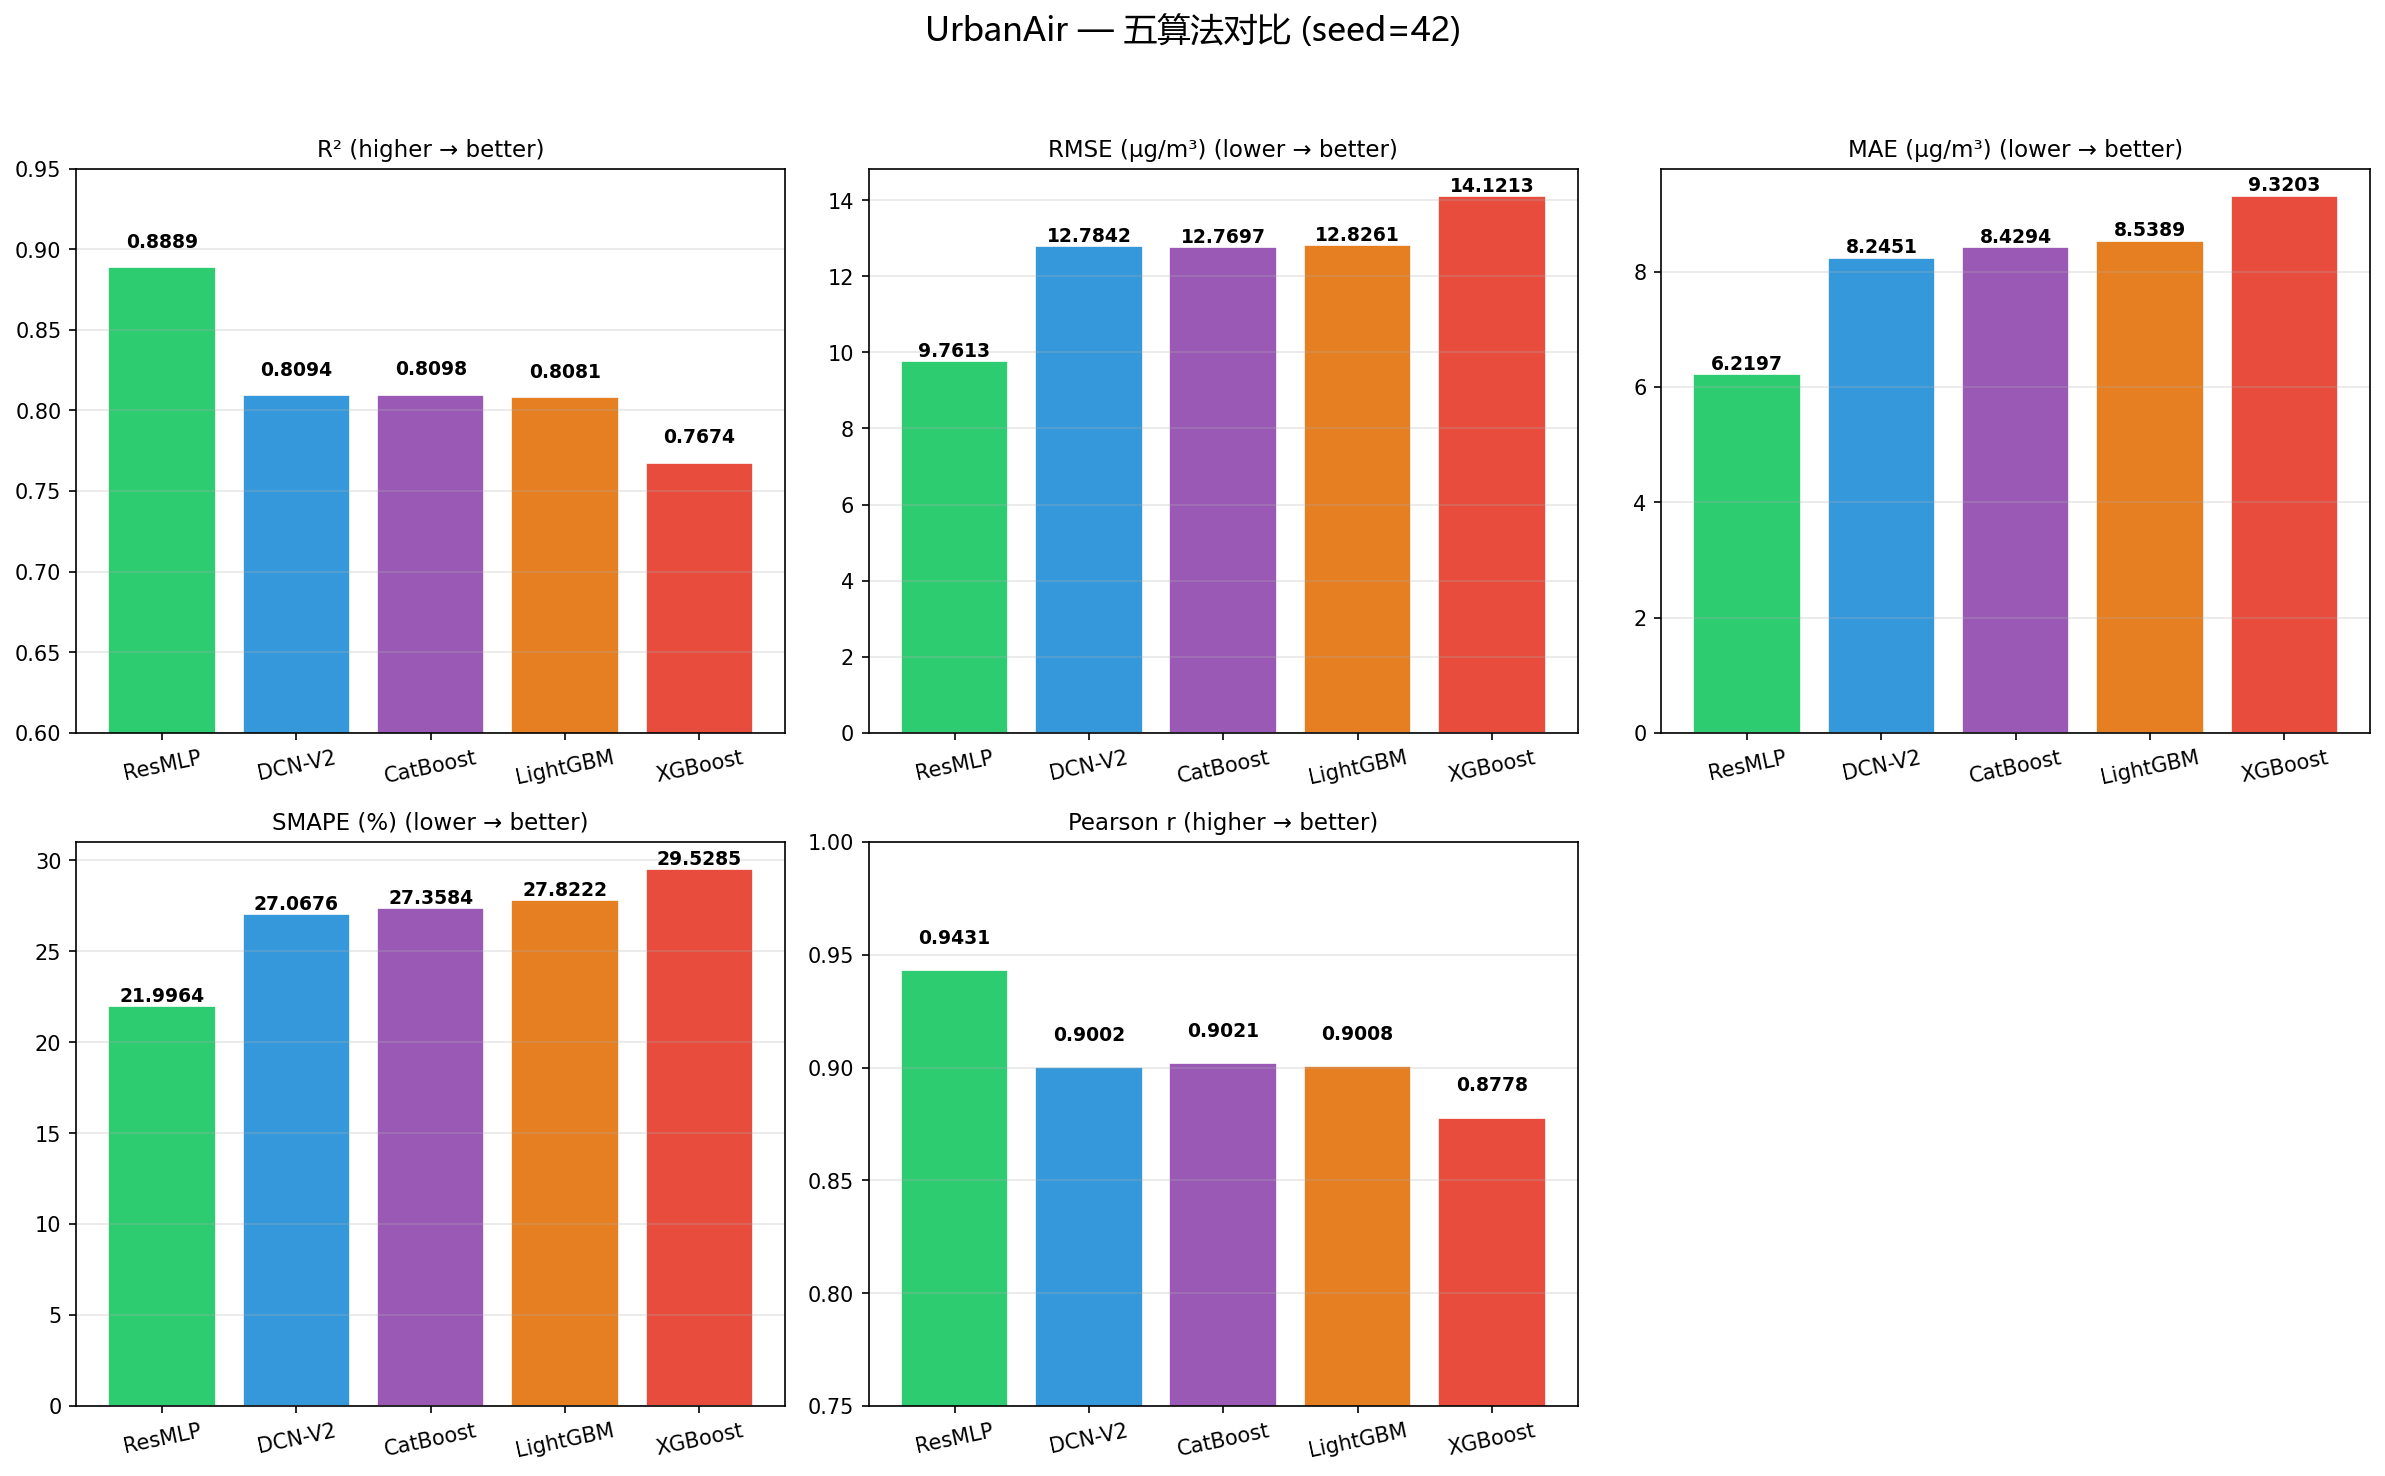
\includegraphics[width=0.92\textwidth]{../comparison_chart.png}
  \caption{模型对比可视化结果}
  \label{fig:comparison_chart}
\end{figure}
}{}

从结果可以看出，ResMLP 相对树模型具有明显优势。可能原因包括：第一，经过标准化后的连续气象和 \aod{} 变量适合 MLP 建模；第二，残差结构能够捕捉多变量之间的非线性交互，同时减少深层网络训练不稳定；第三，warmup 和早停策略提高了训练过程的稳定性。相比之下，树模型虽然在表格数据上通常表现稳健，但在该任务中可能受限于气象和 \aod{} 连续变量之间较平滑的函数关系，难以达到 ResMLP 的拟合能力。

若以 RMSE 衡量误差幅度，ResMLP 相比 CatBoost 的平均 RMSE 从 12.61 降至 9.59，下降约 24.0\%；相比 LightGBM 的 12.70 下降约 24.5\%；相比 XGBoost 的 13.96 下降约 31.4\%。在 MAE 上，ResMLP 相比 CatBoost 从 8.40 降至 6.20，下降约 26.2\%；相比 LightGBM 从 8.53 降至 6.20，下降约 27.3\%。这说明 ResMLP 的优势并非只体现在 $R^2$ 这类整体拟合指标上，也体现在具有实际单位含义的误差指标上。

\begin{table}[H]
  \centering
  \caption{ResMLP 相对主要基线模型的误差下降幅度}
  \label{tab:relative_improvement}
  \begin{tabular}{lcc}
    \toprule
    对比基线 & RMSE 下降幅度 & MAE 下降幅度 \\
    \midrule
    CatBoost & 24.0\% & 26.2\% \\
    DCN-V2 & 24.3\% & 24.6\% \\
    LightGBM & 24.5\% & 27.3\% \\
    XGBoost & 31.4\% & 33.3\% \\
    \bottomrule
  \end{tabular}
\end{table}

从部署角度看，ResMLP 的参数量约为 144K，属于轻量级神经网络。它在预测精度上显著领先，同时较小的参数规模也有利于轻量级推理。因此，选择 ResMLP 作为 Web 应用的默认模型，不仅是基于离线指标最优，也是基于交互式系统对响应速度和部署复杂度的要求。

\subsection{特征消融分析}

表\ref{tab:ablation}已经展示了特征组合消融结果。气象+\aod{} 的组合明显优于 OSM 或 RGB 相关组合，表明本任务的核心信息来自大气气溶胶状态与气象扩散条件。这一结论与已有研究对 \aod{}--\pmfine{} 关系的认识一致：\aod{} 反映整层大气气溶胶负荷，而地面 \pmfine{} 受湿度、风速、边界层和沉降过程影响，需要气象变量进行校正\cite{xin2016,zheng2017}。

OSM 和 RGB 特征表现较弱也具有合理解释。OSM 中的道路密度、建筑密度和土地利用比例主要是静态空间属性，难以解释日尺度污染浓度波动；MODIS RGB 反射率更多描述地表状态，而非直接描述大气气溶胶浓度。将这些变量加入气象+\aod{} 后，模型可能引入冗余或噪声特征，从而降低泛化能力。

\subsection{误差特征}

根据本实验误差分析，模型在极端污染事件上存在低估现象。当 \pmfine{} $>150\ \mu g/m^3$ 时，模型偏差约为 $-18.8\ \mu g/m^3$，主要原因是训练集中此类样本仅占 0.3\%。这说明模型整体指标较好并不意味着对所有污染等级都同等可靠。对于低频高污染样本，后续可考虑重采样、分段损失函数、污染等级加权训练或极端事件单独校准，以改善尾部样本表现。

\section{交互式应用实现}

\subsection{推理流程}

RetroAir 的推理应用基于 Streamlit 构建，核心流程见图\ref{fig:inference}。用户在界面选择经纬度和日期后，系统调用 NASA POWER 获取当日气象变量，从 CAMS EAC4 NetCDF 中按最近网格点提取 \aod{} 特征，计算 \texttt{day\_of\_year}，再将特征按训练时保存的 scaler 标准化，输入 ResMLP 模型得到 \pmfine{} 预测值。最后，系统根据空气质量阈值将数值映射为“优、良、轻度污染、中度污染、重度污染、严重污染”等等级。

\begin{figure}[H]
  \centering
  \fbox{
  \begin{minipage}{0.9\textwidth}
  \centering
  用户输入经纬度与日期
  $\rightarrow$ 获取 NASA POWER 气象
  $\rightarrow$ 提取 CAMS \aod{}
  $\rightarrow$ 构造 17 维特征
  $\rightarrow$ ResMLP 预测
  $\rightarrow$ 输出 \pmfine{} 与空气质量等级
  \end{minipage}}
  \caption{RetroAir 推理流程}
  \label{fig:inference}
\end{figure}

\subsection{界面功能}

Web 应用提供以下功能：
\begin{itemize}
  \item \textbf{地图选点：}用户可以通过地图点击或拖动方式选择目标位置；
  \item \textbf{城市快捷选择：}界面预设多个城市坐标，方便快速测试；
  \item \textbf{日期选择：}支持选择 2018 年至 CAMS 最新可用年份范围内的历史日期；
  \item \textbf{一键预测：}系统自动完成特征获取、模型推理和结果展示；
  \item \textbf{特征详情：}用户可展开查看气象与 \aod{} 特征数值，增强结果透明度。
\end{itemize}

\IfFileExists{../streamlit_demo.png}{
\begin{figure}[H]
  \centering
  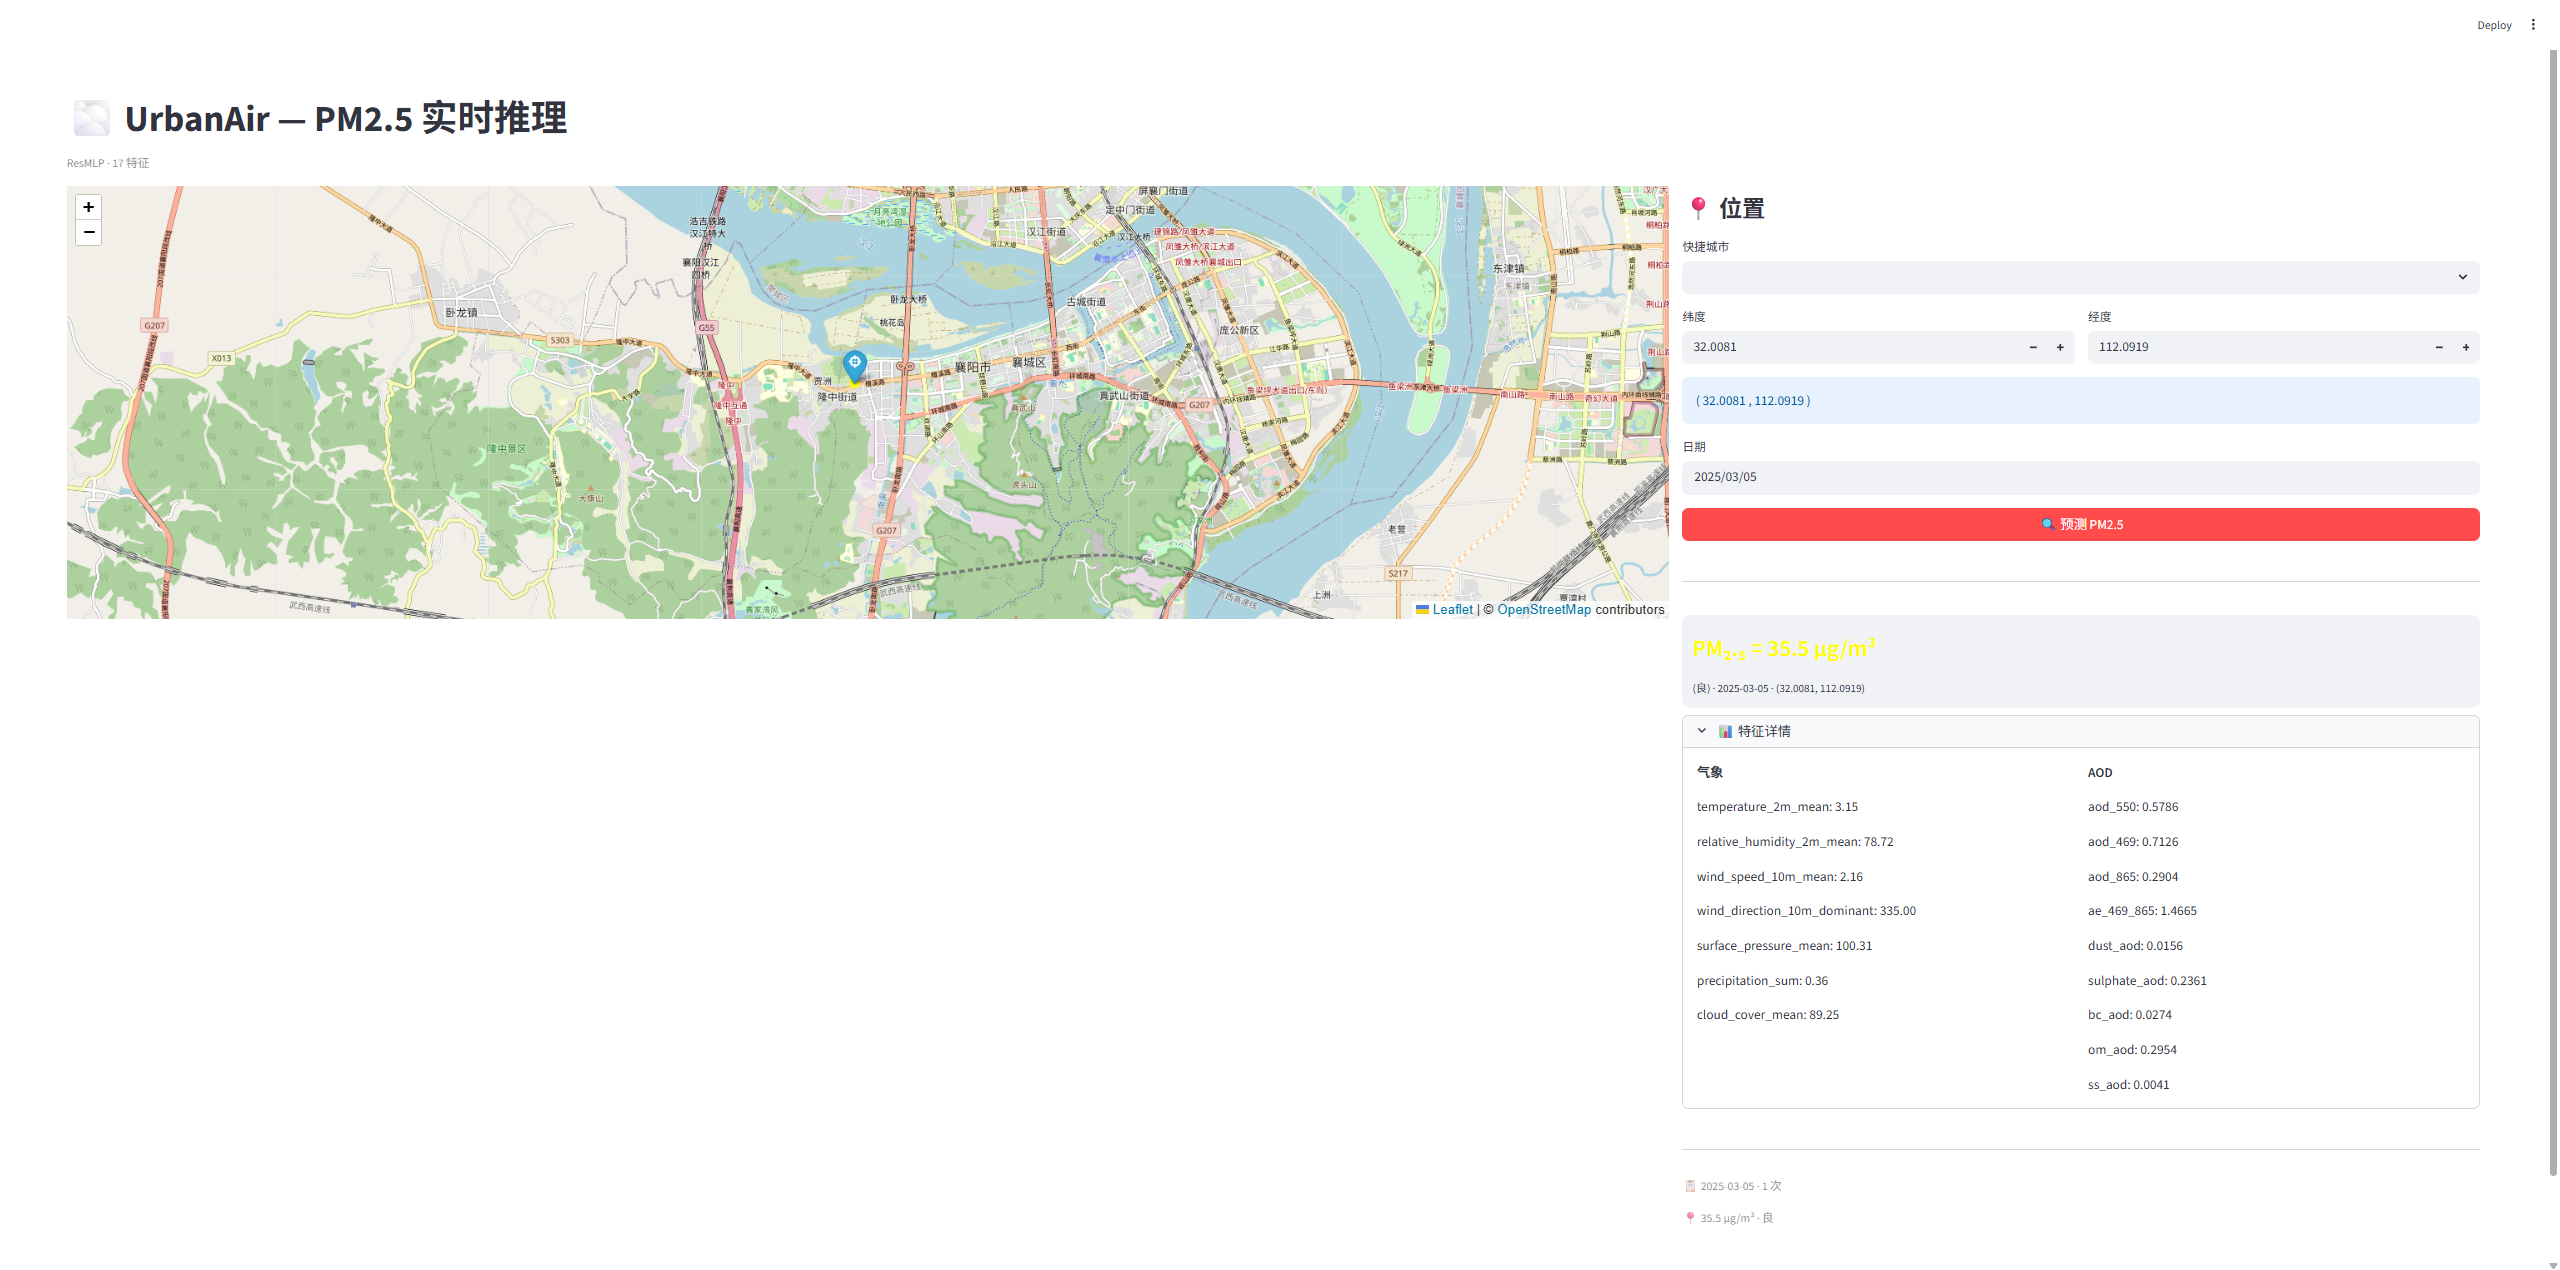
\includegraphics[width=0.92\textwidth]{../streamlit_demo.png}
  \caption{RetroAir Streamlit 交互式推理界面}
  \label{fig:streamlit_demo}
\end{figure}
}{}

该应用将模型结果转化为面向用户的空气质量信息，体现了端到端数据挖掘系统的交付价值。与仅输出离线实验表格相比，交互式界面能够让用户直接选择空间位置和历史日期，观察模型对不同场景的响应。

\subsection{交付物映射}

根据项目要求，选项 C 的核心是构建包含数据处理、模型训练、评估和轻量级交互界面的完整数据挖掘应用。RetroAir 与该要求的对应关系如表\ref{tab:delivery_mapping}所示。数据处理由 AQI、气象和 \aod{} 脚本以及多源合并流程承担；模型训练由多算法训练脚本和 ResMLP 最优模型承担；评估由统一指标、模型对比表和可视化图承担；交互界面由 Streamlit 应用承担。

\begin{table}[H]
  \centering
  \caption{RetroAir 与端到端应用系统要求的对应关系}
  \label{tab:delivery_mapping}
  \begin{tabularx}{\textwidth}{lX}
    \toprule
    要求维度 & RetroAir 对应实现 \\
    \midrule
    数据处理 & 监测站标签获取、NASA POWER 气象获取、CAMS EAC4 \aod{} 提取、三源数据合并 \\
    模型训练 & ResMLP、DCN-V2、CatBoost、LightGBM、XGBoost 等模型训练与保存 \\
    模型评估 & $R^2$、RMSE、MAE、SMAPE、MAPE、Pearson r、Explained Variance 等指标，以及模型对比图 \\
    交互展示 & Streamlit Web 应用，支持地图选点、城市快捷选择、日期选择、预测结果和特征详情展示 \\
    \bottomrule
  \end{tabularx}
\end{table}

从用户视角看，系统输出不只是一个数值预测，还包括空气质量等级、颜色提示、位置与日期信息以及可展开的特征详情。这种设计使模型结果具备解释入口，也便于在答辩演示中展示“输入--处理--输出”的完整链路。

\section{讨论}

\subsection{系统优势}

RetroAir 的主要优势体现在三个方面。首先，系统使用公开可获取的数据源，形成了可复现的数据管道。AKShare、NASA POWER 和 CAMS EAC4 分别提供地面标签、气象变量和气溶胶变量，使项目不依赖封闭数据。其次，模型评估较为系统，既有多算法对比，也有特征消融实验，能够说明最终选择 ResMLP 和气象+\aod{} 特征组合的原因。第三，项目完成了从数据到应用的闭环，能够通过轻量级 Web 界面展示推理结果，符合端到端应用系统开发的目标。

\subsection{局限性}

系统仍存在若干局限。第一，CAMS EAC4 的空间分辨率为 0.75°，约 80 km，难以捕捉道路附近、工业点源和街区尺度微环境差异。第二，极端污染样本占比很低，导致模型对高污染事件存在低估。第三，CAMS 数据存在更新滞后，2026 年后的 \aod{} 数据需要等待数据源更新；因此对近期日期的推理需要采用最近可用年份或等待再分析产品发布。第四，随机切分能够评估整体历史分布拟合能力，但若要评估严格的未见城市或未见站点泛化能力，还需要额外设计跨城市留一验证或空间阻断验证。

\subsection{有效性威胁}

作为审慎的数据挖掘研究，还需要区分模型效果和系统有效性的潜在威胁。首先，标签来自地面监测站，模型学习到的是监测站位置附近的 \pmfine{} 统计规律；当应用到地形、排放结构或气象条件显著不同的区域时，外推误差可能增加。其次，CAMS EAC4 的 \aod{} 是再分析产品而非地面观测，虽然具有全球覆盖优势，但空间分辨率较粗，且与站点尺度污染浓度之间存在尺度差异。再次，本项目统一模型对比采用随机切分，能够评价总体样本分布下的预测能力，但不能完全替代严格的空间外推实验。

这些有效性威胁并不否定系统的实验结果，而是限定其解释范围：本文的结论应理解为“在 8 城市、310,756 样本、气象+\aod{}+时间特征和随机切分设置下，ResMLP 取得最优表现”。对于真正面向全国或全球生产部署的系统，还需要进一步进行跨城市、跨区域和跨年份验证。

\subsection{改进方向}

后续工作可从数据、模型和应用三个层面推进。数据层面，可引入更高空间分辨率的遥感产品、边界层高度、人口密度、道路交通强度等动态或半动态变量；模型层面，可探索分污染等级建模、极端事件加权损失、时空图神经网络或集成校准方法；应用层面，可加入批量点位预测、结果下载、历史趋势可视化和模型不确定性提示，使系统更适合环境健康研究和政策分析场景。

\section{结论}

本文围绕“端到端应用系统开发”目标，设计并实现了 RetroAir 历史 \pmfine{} 回顾性推断系统。系统融合 AKShare 监测站标签、NASA POWER 气象数据和 CAMS EAC4 气溶胶再分析数据，构建 17 维气象+\aod{}+时间特征体系，并完成数据处理、模型训练、统一评估和交互式应用展示。实验表明，在 8 城市 310,756 个样本和 10 个随机种子重复实验设置下，ResMLP 取得最优平均预测性能，$R^2$ 为 $0.8929\pm0.0031$，RMSE 为 $9.59\pm0.14\ \mu g/m^3$，优于 CatBoost、DCN-V2、LightGBM 和 XGBoost 等对比模型。消融实验进一步说明，气象与 \aod{} 是本任务中最关键的特征来源，加入 OSM 或 MODIS RGB 未带来增益。

总体而言，RetroAir 验证了利用多源公开环境数据和机器学习模型推断无站点地区历史 \pmfine{} 的可行性。项目不仅完成了数据挖掘算法实验，也将模型能力封装为可交互的 Web 应用，形成了从数据采集到结果展示的完整工程闭环。

\begin{thebibliography}{99}

\bibitem{who2021}
World Health Organization. \textit{WHO global air quality guidelines: particulate matter (PM2.5 and PM10), ozone, nitrogen dioxide, sulfur dioxide and carbon monoxide}. 2021. \url{https://www.ncbi.nlm.nih.gov/books/NBK574591/}

\bibitem{mee2020}
中华人民共和国生态环境部. 《对十三届全国人大三次会议第6307号建议的答复》. 2020. \url{https://www.mee.gov.cn/xxgk2018/xxgk/xxgk13/202012/t20201201_810823.html}

\bibitem{holloway2023}
Holloway, T., et al. \textit{Satellite Monitoring for Air Quality and Health}. NASA Technical Reports Server, 2023. \url{https://ntrs.nasa.gov/api/citations/20230000905/downloads/Holloway_review_satellite%20monitoring%20for%20air%20quality%20and%20health.pdf}

\bibitem{cams}
Copernicus Atmosphere Monitoring Service / ECMWF. \textit{CAMS global reanalysis (EAC4)}. \url{https://ads.atmosphere.copernicus.eu/datasets/cams-global-reanalysis-eac4}

\bibitem{nasa_power}
NASA POWER Project. \textit{Daily API Documentation}. \url{https://power.larc.nasa.gov/docs/services/api/temporal/daily/}

\bibitem{xin2016}
Xin, J., et al. \textit{The observation-based relationships between PM2.5 and AOD over China}. Journal of Geophysical Research: Atmospheres, 2016. \url{https://doi.org/10.1002/2015JD024655}

\bibitem{zheng2017}
Zheng, Y., et al. \textit{Analysis of influential factors for the relationship between PM2.5 and AOD in Beijing}. Atmospheric Chemistry and Physics, 2017. \url{https://acp.copernicus.org/articles/17/13473/2017/}

\bibitem{wei2019}
Wei, J., Huang, W., Li, Z., Xue, W., Peng, Y., Sun, L., \& Cribb, M. \textit{Estimating 1-km-resolution PM2.5 concentrations across China using the space-time random forest approach}. Remote Sensing of Environment, 2019. \url{https://doi.org/10.1016/j.rse.2019.111221}

\bibitem{li2017}
Li, L., et al. \textit{Mining Public Datasets for Modeling Intra-City PM2.5 Concentrations at a Fine Spatial Resolution}. Proceedings of the ACM SIGKDD International Workshop on Urban Computing, 2017. \url{https://pmc.ncbi.nlm.nih.gov/articles/PMC5841919/}

\end{thebibliography}

\appendix
\section{团队分工声明}

本项目由黄一和、夏浩博、黄迪、许君达四名成员协作完成。团队按照数据工程、算法实现、实验评估和工程部署四个模块进行分工，并通过统一的数据格式、脚本入口和模型文件路径进行协作。各成员的具体贡献见表\ref{tab:team_contribution}。

\begin{table}[H]
  \centering
  \caption{团队成员分工与贡献声明}
  \label{tab:team_contribution}
  \small
  \begin{tabularx}{\textwidth}{llXc}
    \toprule
    成员 & 角色 & 主要工作内容与对应交付物 & 工作量占比 \\
    \midrule
    黄一和 & 算法核心 &
    负责 CAMS EAC4 \aod{} 特征提取模块与深度学习建模部分。具体包括设计并实现 \texttt{03\_fetch\_aod.py} 中的 NetCDF 读取、站点最近网格匹配、日均 \aod{} 特征提取和 Angstrom 指数计算；在 \texttt{scripts/models/nn\_defs.py} 中实现 ResMLP、DCN-V2、FT-Transformer 等神经网络结构；配合 \texttt{scripts/common/torch\_utils.py} 完成 PyTorch 训练流程、warmup 学习率调度和早停策略；负责深度学习模型训练与调优，并参与报告中模型方法、实验结果和局限性分析相关章节撰写。 & 25\% \\
    夏浩博 & 数据工程 &
    负责地面监测站 \pmfine{} 标签、气象数据和多源融合数据集构建。具体包括实现 \texttt{01\_fetch\_aqi.py} 中的 AKShare 真气网监测站数据抓取、站点名称规范化和经纬度清单关联；实现 \texttt{02\_fetch\_weather.py} 中的 NASA POWER 气象数据批量下载、Open-Meteo 兜底和本地缓存机制；实现 \texttt{04\_merge\_data.py} 与 \texttt{05\_merge\_to\_final.py} 中的三源数据合并、去重、缺失值过滤和多城市数据集汇总；参与报告中数据来源、数据处理与特征工程章节撰写。 & 25\% \\
    黄迪 & 实验评估 &
    负责树模型实现、超参数设置、多算法统一对比和特征消融实验。具体包括实现 \texttt{scripts/models/train\_catboost.py}、\texttt{train\_lightgbm.py}、\texttt{train\_xgboost.py} 等树模型训练入口；在 \texttt{06\_compare\_algorithms.py} 中整合 ResMLP、DCN-V2、CatBoost、LightGBM 和 XGBoost 的统一训练、评估、指标保存和对比图生成流程；设计并执行 OSM、MODIS RGB、气象和 \aod{} 特征组合消融实验；负责模型对比表、消融结果和误差分析相关报告内容。 & 25\% \\
    许君达 & 工程部署 &
    负责推理管线、交互式 Web 应用、文档和最终交付整合。具体包括实现 \texttt{scripts/common/data\_utils.py} 中的数据加载、标准化、随机切分和评估指标函数；实现 \texttt{scripts/inference.py} 中的模型加载、在线气象获取、本地 \aod{} 提取、特征组装和 \pmfine{} 预测封装；开发 \texttt{app.py} 中基于 Streamlit、Folium 和地图组件的交互式界面；维护 \texttt{README.md}、依赖说明、运行说明和演示材料，并参与报告中系统设计、交互式应用实现和交付物映射章节撰写。 & 25\% \\
    \bottomrule
  \end{tabularx}
\end{table}

从交付边界看，夏浩博负责输出可复用的多源训练数据集，黄一和负责输出深度学习模型结构与训练权重，黄迪负责输出多算法评估结果与特征选择结论，许君达负责将数据、模型和推理逻辑集成为可运行的用户界面和项目文档。上述分工覆盖了项目要求中的数据处理、模型训练、模型评估和交互展示四个核心环节，且各成员均有明确的代码文件、报告章节和可量化工作量对应关系。

\end{document}

